\documentclass{thesis}
% Damit die Verwendung der deutschen Sprache nicht ganz so umst\"andlich wird,
% sollte man die folgenden Pakete einbinden: 
\usepackage[latin1]{inputenc}% erm\"oglich die direkte Eingabe der Umlaute 
\usepackage[T1]{fontenc} % das Trennen der Umlaute
\usepackage{cite}
%\def\BibTeX{{\rm B\kern-.05em{\sc i\kern-.025em b}\kern-.08em
 %   T\kern-.1667em\lower.7ex\hbox{E}\kern-.125emX}}
\usepackage[german,german]{babel} % hiermit werden deutsche Bezeichnungen genutzt und 
                     % die W\"orter werden anhand der neue Rechtschreibung 
		     % automatisch getrennt.  
\title{Trapping and Beamloading in hybrid Plasma Wakefield Accelerator schemes}
\author{Alexander Knetsch}

\date{\today}
% Hinweis: \title{um was auch immer es geht}, \author{wer es auch immer 
% geschrieben hat} und  \date{wann auch immer das war} k\"onnen vor 
% oder nach dem  Kommando \begin{document} stehen 
% Aber der \maketitle Befehl mu\ss{} nach dem \begin{document} Kommando stehen! 

\begin{document}

\maketitle
\tableofcontents


\section{The history of wakefield acceleration}
Tajima Dawson great Idee, MTV bubble regime, same time PWFA von Rosenzweig... first linear measurements for PWFA
\section{Plasma physics}
There are several definitions of a plasma, but one of the most appealing one that we will follow in this work can be found in the classic 
textbook by Francis F. Chen:
"A plasma is a quasineutral gas of charged and neutral particles which
exhibits collective behavior" \cite{Chen_book_Plasma}.
Regarding the gas types we will conveniently assume them to be electrons, ions and neutral atoms and comment that other particles as well can fit the definition of a plasma, but such exotic compositions are beyond the scope of this work.
As plasmas are electromagnetically interacting a common and very useful way to describe it on a fundamental level is with the help of the Maxwell equation.
\begin{equation}
\label{eqn:Maxwell}
\vec{\nabla} \vec{E} = \frac{\rho}{\epsilon_0},\	\vec{\nabla}\vec{B} =0\,	\vec{\nabla}\times\vec{E}=-\frac{\partial \vec{B}}{\partial t},\ 
 \vec{\nabla}\times \vec{B}=\mu_0\vec{j}+\mu_0\epsilon_0\frac{\partial \vec{E}}{\partial t}.
\end{equation}
$\vec{E}$ and $\vec{B}$ are the electric and magnetic field and  $\vec{j}$ and $\rho$ is the current density and charge density.
$\epsilon_\mathrm{m}$ and $\mu_\mathrm{m}$ are the vacuum  dielectric constant and the vacuum permeability.
In a fluid description it makes also sense to assume that no particles are created or destroyed which is the origin of the 
continuity equation 
\begin{equation}
\frac{\partial \rho}{\partial t} + \vec{\nabla}(\rho \vec{v})=0.
\end{equation}




\subsection*{Plasma frequency}
Electrons and ions in a plasma can be described as two fluids, each following the fluid dynamics and interacting via the Maxwell Equations and collisions.

If the electron fluid is displaced with respect to the ion fluid this leads to strong electric fields, acting upon both as a restoring force, but as $m_\mathrm{i}>>\mE$, the electron response is much quicker which is why these kind of plasma oscillations are dominated by the electrons, while the ions can be considered inert.

Starting from equation (\ref{eqn:Poisson_plasma}) with the relation of the electric field and its potential being $\vec{E}=-\nabla \Phi$ 
\begin{equation}
\epsilon_0 \nabla \vec{E}=\qE (n_\mathrm{i}-\nE)
\end{equation}
becomes for small perturbations $n'=\nE+\delta n$
\begin{equation}
\epsilon_0 \nabla \vec{E}=\qE \delta n).
\end{equation}
The solution to this differential equation is a harmonic density oscillation 
\begin{equation}
n(x,t)=\delta n \exp(i(kx-\wP t)).
\end{equation}
The characteristic frequency of this oscillation 
\begin{equation}
\omega_\mathrm{p}=\sqrt{\frac{n_\mathrm{e}q_\mathrm{e}^2}{\epsilon_0 m_\mathrm{e}}}
\end{equation}
is called the \textit{Plasma frequency} and is one of the most important parameters in plasma physics. 
In the field of PWFA it is convenient to also consider the wavelength associated with the plasma oscillations, 
the \textit{Plasma wavelength}
\begin{equation}
\lP=2\pi\frac{\wP}{c}.
\end{equation}

Typical values for example for a plasma density $\nE=1\times10^{17}\mathrm{cm}^{-3}$ are

\begin{align*}
\wP &\approx 56400 \sqrt{\nE [\mathrm{cm}^{-3}]} \approx 1.8\times10^{18}\ 1/s\\
\lP & \approx 105.6 /\sqrt{\nE [10^{17} \mathrm{cm}^{-3} ]} [\mu\mathrm{m}] = 105.6\ \mu\mathrm{m}.
\end{align*} 

\subsection*{Debye Shielding}
The concept of \textit{quasi-neutrality} roots in the shielding behavior of the ions and electrons of charges inside the plasma. 
A positive net charge e.g. originating from a difference in ion density $n_\mathrm{i}$ and electron density $n_\mathrm{e}$ at a temperature $T$
would attract electrons and lead to an electron distribution 
\begin{equation}
f(u) \propto \exp(-\frac{1}{2}\mE v^2+\qE/( k_\mathrm{B}T)).
\end{equation}

With the Poisson Equation 
\begin{align}
\label{eqn:Poisson_plasma}
\epsilon_0 \frac{d^2\Phi}{dx^2}&=-\qE(\nE-n_\mathrm{i})\\
&=\qE \nE (\exp(\qE\Phi/(k_\mathrm{B}T))-1)\\
&\approx \qE\nE(\qE\Phi/(k_\mathrm{B}T)+...)
\end{align}
we can now derive the potential in the plasma
\begin{equation}
\Phi = \Phi_0\exp(-|x|/\lambda_\mathrm{D})
\end{equation}
with the information about the range of the shielded Coulomb field embedded in the Debye Radius
\begin{equation}
\lambda_\mathrm{D}=\sqrt{\frac{\epsilon_0 k_\mathrm{B}T}{n_\mathrm{e}\qE^2}}.
\end{equation}
We can see that a plasma with an edge length $L>>\lambda_\mathrm{D}$ would have its Coulomb fields shielded and appear to an outside observer to be charge-neutral. 




%\subsection{time scales}
%scattering can be talked about

%\subsection{plasma definition}
%There are different types of plasm<as, but we are only handling with thin, cold  weakly coupled plasmas
\subsection{electromagnetic waves in plasmas}
It is worth noting that the Debye Shielding assumes a thermalized plasma and is not the right idea of a plasma reaction to a rapid change in charge on a femtosecond timescale. 
The more appropriate figure of merit in that case is the depth an electromagnetic wave 

with frequency $\omega$ can permeate the plasma fluid.

This can be calculated by applying the Maxwell equations \ref{eqn:Maxwell} so that one gets the differenctial equation.
\begin{equation}
\label{eqn:Laser_prop_DGL}
\vec{\nabla}(\vec{\nabla})\vec{E}-\Delta \vec{E}/(\epsilon_0 \mu_0)=\frac{1}{\epsilon_0}\frac{\partial \vec{j}}{\partial t}+\frac{\partial^2 \vec{E}}{\partial t^2}
\end{equation}
In plasma the current density is not 0, but 
$\frac{\nE \qE^2}{?}$
Equation ... can be solved with an exponential Ansatz
\begin{align}
\vec{E}&=E_0 e^{ikx-i\omega t}\\
\end{align}
leading to a dispersion relation
\begin{equation}
\omega^2 = c^2 \kP^2+\wP^2
\end{equation}

the skin depth 
\begin{equation}
\kP^{-1}=\frac{c}{\sqrt{\wP^2-\omega^2}}.
\end{equation}
%
%As Lasers are going to play a significant role in the ionization, plasma shape creation and the injection of electron beams we have to get an overview over the assumptions taken into account and problems that can be faced by applying shortpulse laser pulses for this matter. 
%
%To describe laser propagation in a medium a fundamental approach is to start with the Maxwell equations
%
%dispersion relation needs to be talked about. Especially the dispersion relation of lasers during ionization should get some insight here. One has to look into ionization defocussing.  
%


%\subsection{laser ionisation description}
%(see diss by Ihar Shchatsinin FU Berlin)


\subsection{Underdense ionization with ultrashort laser pulses}

Original ADK paper: \cite{ADK_original}
\begin{equation}
w=\omega_\mathrm{at}\Big(\frac{3}{} \Big)
\end{equation}
In \cite{bruhwiler2003PoP} Bruhwiler et al. have developed an approximated equation which is optimated for using it in numerical operations such as PIC codes, where the ADK ionization rate is 
\begin{equation}
W_\mathrm{ADK}=1.52\times 10^{15}\frac{4^{n^*}\xi_\mathrm{ion}[eV]}{n^*\Gamma(2n^*)}\Big(20.5\frac{\xi_\mathrm{ion}^{3/2}[eV]}{E[GV/m]}\Big)^{2n^*-1}\times \exp(-6.83\frac{\xi_\mathrm{ion}^{3/2}[eV]}{E[GV/m]})
\label{eqn:ADK_Bruhwiler}
\end{equation}
for an element to the ionization level $Z$ with its ionization energy $\xi_\mathrm{ion}$.
$n^*\approx 3.69Z/\xi_\mathrm{ion}$ is the effective principal quantum number.
A list of ionization energies can be found in \cite{Kelly_1982_Ion_Energies}.
The actual ionization ratio of a gas with plasma density for dull ionization $n_0$ is then

\begin{equation}
\frac{\nE(t)}{n_0} =1-\exp\Big(-\int \limits_{-\infty}^t W_\mathrm{ADK}(t')dt'\Big).
\end{equation}
As we treat ultrashort pulses, the time scales in which the ionization occurs is comparable to that of the laser pulse rms length $\tau$. We assume e.g. a laser pulse linearly polarized in y. 
The electric field can be approximated by the envelope of the laser electric field to 
\begin{equation}
E_{y}(t)=E_0\exp(-\frac{t}{2\tau^2}),
\end{equation}
because the ADK theory averages over DC fields.

\begin{equation}
E_{x}(r,z,t)=E_0\frac{w_0}{w(z)}\exp(-\frac{r^2}{w(z)^2})\exp(-\frac{t}{2\tau^2})
\end{equation}

$w(z)=w_0(1+(\frac{z}{z_0})^2)^{1/2}$ is the beam waist at longitudinal position $z$ and $z_0=\pi w_0^2/\lambda$ is the Rayleigh length.

\begin{equation}
\nE(r,z,t) = n_0 \Big(1-\exp\Big(-\int \limits_{-\infty}^t W_\mathrm{ADK}(E_{x}(r,z,t'))dt'\Big)\Big).
\end{equation}

\begin{figure}
\centering
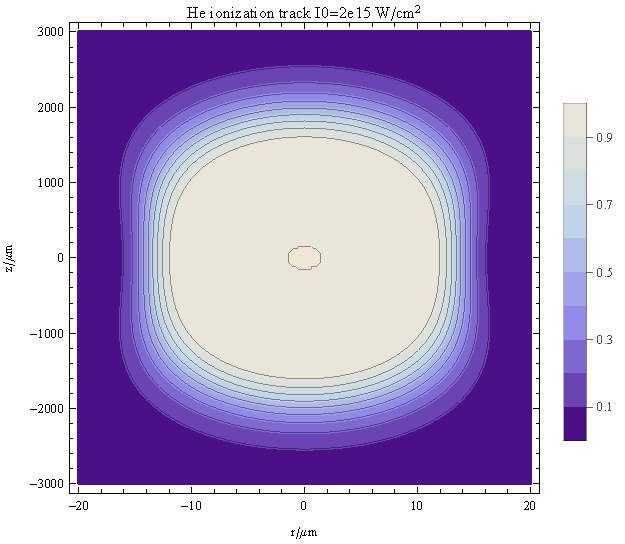
\includegraphics[width=0.6\textwidth]{theory/images/raw/Ionization_Torch_contourplot.pdf}
\caption{He Ionization ratio by a 1 mJ Gaussian laser pulse with waist $w_0=20\ \mu m$ and $\tau = 70\ \mathrm{fs}$ FWHM pulse length}
\label{img:Torch_contourplot}

\end{figure}


%\subsection{waves in plasmas}
%So far everything still flows niocely with working along Chen and Mulser. However now the turn needs to be taken.
%The reason is wavebreaking

\section{PWFA theory}
\subsection{History of PWFA}
A short historic overview is given. 
Maybe mention landau damping? Then of course, Tajima,Dawson. Also MTV and Rosenzweig should be mentioned.
\section{The linear regime}
Herleitung by esarey \cite{RevModPhys.81.1229}


\begin{equation}
E_\xi=4\pi \int_0^\xi \rho{\xi'}\cos(\kP(\xi-\xi'))d\xi
\end{equation}
The transformer ratio $R_\mathrm{trans}=\frac{E_\mathrm{max}^+}{E_\mathrm{max}^-} $ in PWFA is defined as
the ratio of the maximum accelerating electric field
behind the driving bunch, $E_\mathrm{max}^+$, to the maximum decelerating $E_\mathrm{max}^-$
electric field acting upon drive beam electrons. Experimentally the transformer ratio is comparably easy access-able if one assumes the acceleration length for the witness beam and deceleration length for the drive beam to be equal and that the  witness beam is in accelerated at the peak accelerating field.
Then it can be observed in the electron energy spectrum as the maximum energy gain of the witness beam divided by the maximum energy loss of the drive beam. In that sense the transformer ratio is a measure of efficiency with which the drive electron beam can transfer energy to the witness electron beam. 
In the linear regime for a Gaussian drive beam 
In \cite{PhysRevLett.56.1252} it is calculated and simulated that the transformer in the linear regime, which is otherwise limited to $R_\mathrm{trans}\leq 2$ for a symmetric drive beam current profile \cite{bane1984wake}, can reach up to $R_\mathrm{trans}\approx 6.12$ by applying a triangular shaped drive beam current.
\section{The blowout regime}
\label{sec:Blowout_regime}


Wavebreaking limit: \begin{equation}
E_\mathrm{WB}=cm_\mathrm{e}\omega_\mathrm{P}/q_\mathrm{e}\simeq 96 \sqrt{n_\mathrm{e}(\mathrm{cm}^{-3})}
\end{equation}
Wavebreaking gives us the the ideal way to go from plasma description to blowout description.

\section{Descriptions for the blowout regime}
Lotov, Suk, breakdown of fluid theory
Q-tilde and resonant wake excitation.


\section{Accelerator physics}
In the previous chapters we examined the physics of the beam driven plasma wake excitation. 
The ultimate goal as presented in this work is to advantageously make use of the fields in order to inject and accelerate a high quality secondary electron beam, which is conventionally called the witness beam. If there are no substantial advantages between  using the witness over the drive beam for a given application, it might not be worth the effort beyond a scholastic interest.
In this section we will explain the basic electron beam behavior in an accelerator and from that determine the most important parameters. 
\subsection{Single particle movement}

We start with the 
\begin{equation}
\vec{F}=\frac{d\vec{p}}{dt}=q(\vec{E}+\frac{\vec{v}}{c}\times\vec{B})
\end{equation}

Similar to the assumptions made in par-axial optics the electron can be expected to 
follow a straight trajectory in the absence of any deflecting or accelerating force and any small change in that trajectory 
can be expressed in a number of linear changes. 
As in par-axial optics this gives the possibility to describe the electron beam trajectory with linear transformations, represented by a matrix formalism.
This idea can be extrapolated to the entire phase-space information of an electron, so that equation
\begin{equation}
\label{eqn:R_Matrix}
\begin{split}
\Phi_\mathrm{f}&=\hat{R} \Phi_\mathrm{i} \\
\begin{pmatrix}
x_\mathrm{f}\\
x'_\mathrm{f}\\
y_\mathrm{f}\\
y'_\mathrm{f}\\
z_\mathrm{f}\\
\delta_\mathrm{f}\\
\end{pmatrix}
&=
\begin{pmatrix}
R_{11}&R_{12}&R_{13}&R_{14}&R_{15}&R_{16}\\
R_{21}&R_{22}&R_{23}&R_{24}&R_{25}&R_{26}\\
R_{31}&R_{32}&R_{33}&R_{34}&R_{35}&R_{36}\\
R_{41}&R_{42}&R_{43}&R_{44}&R_{45}&R_{46}\\
R_{51}&R_{52}&R_{53}&R_{54}&R_{55}&R_{56}\\
R_{61}&R_{62}&R_{63}&R_{64}&R_{65}&R_{66}\\
\end{pmatrix}
\begin{pmatrix}
x_\mathrm{i}\\
x'_\mathrm{i}\\
y_\mathrm{i}\\
y'_\mathrm{i}\\
z_\mathrm{i}\\
\delta_\mathrm{i}\\
\end{pmatrix}
\end{split}
\end{equation}

describes a complete linear transformation of an electron's phase space vector as a conservative force acts upon it, with the spatial components $x,y,z$, the transverse momenta $x'=\frac{p_\mathrm{x}}{p_\mathrm{z}},y'=\frac{p_\mathrm{y}}{p_\mathrm{z}}$ and the deviation  $\delta=\frac{\delta p_\mathrm{z}}{p_\mathrm{z}}$ from the design momentum $p_\mathrm{z}$
The matrix $\mathbf{R}_\mathrm{m,n}= \frac{\delta \Phi_\mathrm{n}}{\delta \Phi_\mathrm{n}}$ is the Jacobian of this transformation and as that it requires $\mathrm{det}(\hat{R})=1$.


Wiedemann:\cite{Wiedemann_accelerator}


 Jamies book: \cite{Book_Fundamentals_Rosenzweig}
\subsection{Liouville Theorem}
When now considering an entire bunch of electrons it comes in handy to describe it as a smooth phase space distribution
$f(\vec{r},\vec{p})$, which is conventionally normalized so that  
\begin{equation}
\label{eqn:f_int_1}
\int^{\infty}_{-\infty}f(\vec{r},\vec{p})d\vec{r}d\vec{p}=1 .
\end{equation}

The Liouville Theorem states that if only conservative forces are applied to the bunch the total phase volume occupied by the distribution stays constant. This is mathematically equivalent to any transformation that maintains condition (\ref{eqn:f_int_1}), which can be expressed by Jacobian transformations of the kind described by equation (\ref{eqn:R_Matrix}).
Of course $\hat{R}$ does not need to act upon the entire 6D-Phase space. In fact it is common to reduce the analysis and describe only changes in the transverse phase space, the so called \textit{trace space}, as the planes are mathematically independent and often beam-optics that only influence one plane such as quadropoles or dipoles are applied.

In order to obtain a measure of the actual phase space volume the statistical moments of the distribution can be determined by evaluating the integral 
\begin{equation}
<x^n>=\int_{-\infty}^{\infty}f(\vec{r},\vec{p})x^n dx.
\end{equation}
%with the total time differentiate
%\begin{align}
%\frac{d f}{dt}&=\frac{\partial f}{\partial t}+\sum_i \frac{dx_i}{dt}\frac{\partial f}{\partial x_i}+\frac{dp_i}{dt}\frac{\partial f}{\partial p_i}
%&=\frac{\partial f}{\partial t}+\sum_i()
%\end{align}
\subsection{Courant-Snyder coefficients, brightness and emittance}
Courant and Snyder with their summary paper \cite{COURANT1958} have set the standard for defining the phase space volume in the trace space with an ellipse equation for its boundary
\begin{equation}
\label{eqn:CourandSnyderEllipse}
\gamma <x^2>+2\alpha <x> <x'>+\beta <x'^2> =\epsilon.
\end{equation}
\begin{equation}
\alpha =\frac{<x^2>}{\epsilon}, \gamma=\frac{<x'^2>}{\epsilon}, \alpha=\frac{<xx'>}{\epsilon}
\end{equation}
are the so called \textit{Courant Snyder parameters} and $\epsilon$ is the trace space emittance. 
As $f(\vec{r},\vec{p})$ is considered to be smooth function, it might as well consist of a distribution that only approaches 0 so that it is difficult to draw a absolute volume edge as illustrated in figure (\ref{img:TraceSpace}).
Because of this and for the sake of simplicity in comparing the value with experimental data, it is useful to work with the rms values. So the \textit{rms trace space emittance} according to \cite{PRSTAB_Emittance_Floettmann} is
\begin{equation}
\epsilon_\mathrm{tr,rms}=\sqrt{<x^2><x'^2>-<xx'>^2}.
\end{equation}
This can additionally be normalized to the \textit{normalized rms trace space emittance} into the form
\begin{equation}
\label{eqn:NormTraceSpaceEmitt}
\epsilon_\mathrm{n,tr,rms}=\frac{p_\mathrm{z}}{\mE c}\sqrt{<x^2><x'^2>-<xx'>^2}
\end{equation} 
so that its value stays current during acceleration.
The emittance is an important value, as it is invariant under conservative transformations and therefore an important 
figure of merit for electron beam quality in general. 
Definition (\ref{eqn:NormTraceSpaceEmitt}) will mostly be applied in the context of this work.
\begin{figure}[htbp]
\begin{center}
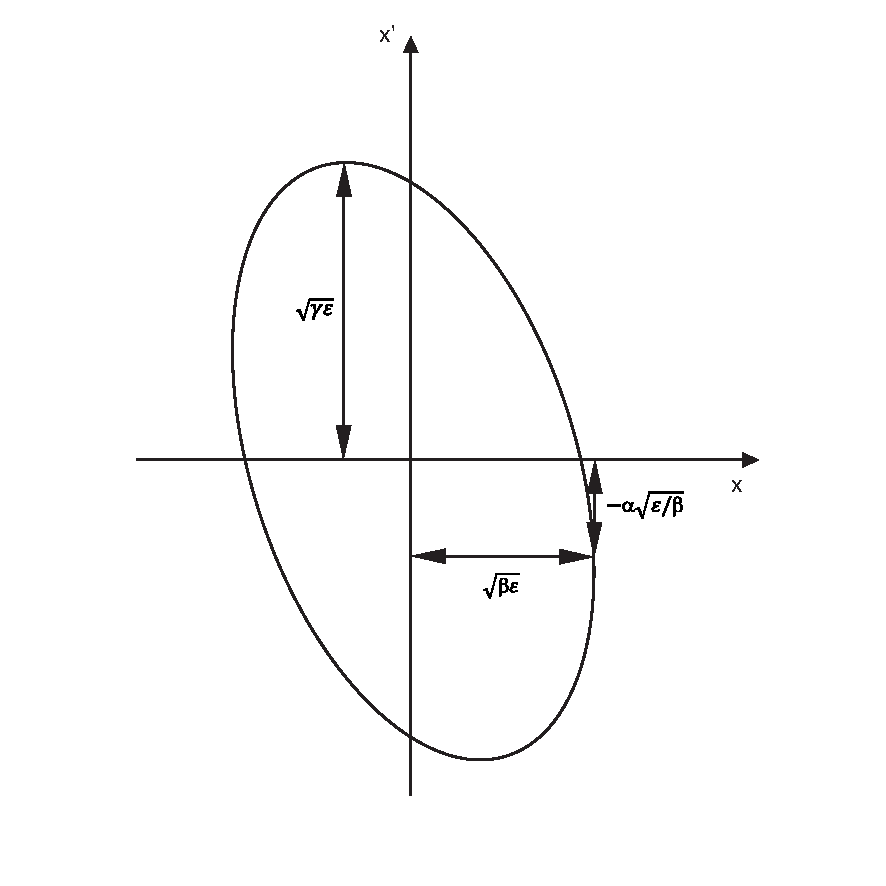
\includegraphics[width=0.6\textwidth]{theory/images/edited/TraceSpaceCourantSnyder.pdf}
\end{center}
\caption{Illustration of the trace space ellipse and its connection to the Courant Snyder coefficients.}
\label{img:TraceSpace}
\end{figure}
As in the forthcoming parts of this work we will have a look at numerical simulations conducted with particle-in-cell (PIC) Simulations, that handle discrete phase space points as electron beam representation instead od a continuum a discrete emittance expression will be used. For that the electron beam moments are sums in the following form.
\begin{align}
<x^2>&=\frac{1}{n} \sum_{i=1}^{n} x_i^2-\frac{1}{n^2}\Big(\sum_{i=1}^{n} x_i\Big)^2\\
<x'>&=\frac{1}{n} \sum_{i=1}^{n}\Big(\frac{p_{x,i}}{p_{z,i}}\Big)^2-\frac{1}{n^2}\Big(\sum_{i=1}^{n}\frac{p_{x,i}}{p_{z,i}}\Big)^2\\
<xx'>&=\Big(\frac{1}{n}\sum_{i=1}^{n}x_i\frac{p_{x,i}}{p_{z,i}}-\frac{1}{n^2}\sum_{i=1}^{n}x_i \sum_{j=1}^{n}\frac{p_{x,i}}{p_{z,j}}\Big)^2
\end{align}


\subsection{Panowsky-Wenzel Theorem}

original paper:  \cite{Panowsky_Wenzel_original}

 \begin{equation}
W_r =\partial_r W_z
\end{equation} 
This theorem is so important, it clearly needs a subsection. But where ?


\section{Electron Trapping in plasma accelerators}
\label{sec:Theory_Trapping}


In order to derive an expression for the trapping condition of a single electron in PWFA, one has to start with the equation of motion for such a single electron. 
\begin{equation}
\vec{F}=\frac{d\vec{p}}{dt}=q(\vec{E}+\frac{\vec{v}}{c}\times\vec{B})
\end{equation}
with the electron charge $q$ electric field $\vec{E}$ and magnetic field $\vec{B}$

This leads to the single particle electron hamiltonian $ H=\gamma m c^2+\Phi$ with the temporal derivative.
\begin{align}
\frac{dH}{dt}&=\frac{d}{dt} (\gamma m_e c^2)+\frac{d}{dt}(q\Phi)\\
&=\vec{v}\frac{d\vec{p}}{dt}+\frac{d}{dt}(q\Phi)\\
&=q\vec{v}(-\nabla \Phi-\frac{\partial \vec{A}}{\partial t})+\frac{\vec{v}\times\vec{B}}{c}+\frac{d}{dt}(q\Phi)\\
&=q(\frac{d}{dt}\Phi-\vec{v}\vec{\nabla}\Phi-\vec{v}\frac{\partial \vec{A}}{\partial t})\\
&=q(\frac{\partial \Phi}{\partial t}-\vec{v}\frac{\partial \vec{A}}{\partial t})
\end{align}

If one assumes now, that the wake fields are constant during the trapping process, then 

\begin{equation}
(\frac{\partial}{\partial t}+v_\mathrm{\phi} \frac{\partial}{\partial z} ) f =   f ( z-v_\mathrm{\phi} t)
\end{equation}\begin{equation}
(\frac{\partial}{\partial t}+v_\mathrm{\phi} \frac{\partial}{\partial z} ) f =0 \ \forall \   f (\vec{r}, z-v_\mathrm{\phi} t)
\end{equation}
which is especially true for the hamiltonian.
\begin{align*}
\frac{d}{dt}H&=q(\frac{\partial \Phi}{\partial t}-\vec{v}\frac{\partial \vec{A}}{\partial t})\\
&=-q v_\mathrm{\phi}(\frac{\partial \Phi}{\partial z}-\vec{v} \frac{\partial \vec{A}}{\partial z}) 
\end{align*}

Since $H-v_\mathrm{\phi}P_z=\mathrm{const.}$

\begin{align}
H-v_\mathrm{\phi}P_z &= \mathrm{const.}\\
\gamma m c^2+\Psi-v_\mathrm{\phi}p_z-v_\mathrm{\phi}qA_z &= \mathrm{const.}\\
\gamma+\frac{q \Phi}{m c^2}-v_\mathrm{\phi} \frac{p_z}{mc^2} &= \mathrm{const.}\\
\gamma - v_\mathrm{\phi} \frac{p_z}{mc^2}- \underbrace{\frac{q}{mc^2}(\Phi-v_\mathrm{\phi}A_z)}_{\bar{\Psi}}  &= \mathrm{const.} 
\end{align}
$\bar{\Psi}$ is the trapping potential, that determines the potential difference for an electron in a potential that moves with a phase velocity $v_\mathrm{\phi}$ with respect to the laboratory frame. It is valid for small as for relativistic velocities.
With the trapping potential one can calculate if an electron inside the plasma wake will be accelerated or not i.e. if electrons will be able to catch up with the wake's velocity during the propagation of the wake or if it will slip out of the potential.
From the prior calculations a general formula can be determined, that compares

\begin{equation}
\label{eqn:Trapping_Potential_Pre}
\Delta \bar{\Psi}= \bar{\Psi}_\mathrm{i}-\bar{\Psi}_\mathrm{f}=\gamma_\mathrm{f}-\gamma_\mathrm{i}-\gamma_f\frac{v_\mathrm{\phi}v_\mathrm{f}}{c^2}+\gamma_\mathrm{i}\frac{v_\mathrm{\phi}v_\mathrm{i}}{c^2} 
\end{equation}

In order to honor the name "trapping potential" i.e. to apply this derivation to make predictions of the electron trapping behavior in the plasma wake, it is necessary to define a trapping condition. 
An obvious and conventional choice is that an electron should catch up with the wake's velocity so that 
$v_\mathrm{f}=v_\mathrm{\phi}$.
Equation (\ref{eqn:Trapping_Potential_Pre}) consequently simplifies to 
\begin{align}
\label{eqn:Trapping_Potential_Raw}
\Delta \bar{\Psi}&= \gamma_\mathrm{\phi}-\gamma_\mathrm{i}-\gamma_\mathrm{\phi}\frac{v_\mathrm{\phi}^2}{c^2}+\gamma_\mathrm{i}\frac{v_\mathrm{\phi}v_\mathrm{i}}{c^2} 
\end{align}
Equation (\ref{eqn:Trapping_Potential_Raw}) can be further separated into different physical cases:
\subsection*{luminal wakefield, electron injected  at rest}
In this case the plasma wake travels with a phase velocity near the speed of light, which is the case for beam-driven scenarios with high $\gamma$ driver beams ($v_\mathrm{\phi} \approx c$), and electrons starting inside the wake initially at rest ($v_\mathrm{i} \approx \ 0$).
Here Equation (\ref{eqn:Trapping_Potential_Raw}) simplifies to
\begin{equation}
\label{eqn:Trapping_Potential_TH}
\Delta \bar{\Psi}=-1
\end{equation}
Examples of this case are the underdense photocathode, or Trojan Horse injection\cite{Hidding_PRL_2012}, or wakefield induced ionization injection\cite{MartinezdelaOssa2014231}.

\subsection*{luminal wakefield, electron injected  with v $\neq 0$}
\begin{equation}
\Delta \bar{\Phi}= -\gamma_\mathrm{i}(1-\frac{v_\mathrm{i}v_\phi}{c^2})\approx -\gamma_\mathrm{i}(1-\frac{v_\mathrm{i}}{c})
\end{equation}
\subsection*{subluminal wakefield, electron injected at rest}

\begin{equation}
\label{eqn:Trapping_Potential_DTH}
\Delta \bar{\Psi}=\gamma_\mathrm{\phi}(1-\frac{v_\mathrm{\phi}^2}{c^2})-1=\gamma_\mathrm{\phi}^{-1}-1
\end{equation}
This formula can for example be applied to ionization injection in LWFA\cite{PakPRL2012} or beam-driven ionization injection schemes in which the wake's phase velocity is retarded such as the Downramp-assisted Trojan Horse (DTH)\cite{DTH}, which this work has as special focus on. In latter case mathematically strictly speaking $\frac{d H}{dt}\neq0 $, but for small changes $\frac{dH}{dt}\approx 0$ during the injection process of the electrons, equation (\ref{eqn:Trapping_Potential_DTH}) can still be applied.

\subsection*{superluminal wakefield}
There are physical situations imaginable in which the wake or at least part of the wake move with a phase velocity faster than the speed of light. This is the case for example when a beam driven wake traverses an electron density upramp.
From the previous deductions it seems obvious, that trapping electrons in such a superluminal wakefield is not possible, as $\gamma_\mathrm{\phi}^{-1}$ becomes complex for $v_\mathrm{\phi}>c$.

However, if the superluminosity is only transient as with a short density upramp, the phase velocity will return to $c$ right after the transition. In this case trpping can be possible, but the mathematic tool presented in this section is insufficient to describe the trapping and the phase velocity after the transition is setting the demand on the potential.
\subsection{Trapping position and bunch compression}
Assuming that the longitudinal wake field 
$\frac{\partial E_\mathrm{z}}{\partial r} = 0 $ for a sufficiently wide radius the trapping behaviour can be seen in 1D only.
In the blowout regime the acceleration gradient is to second order linear in $\xi$ (compare section (\ref{sec:Blowout_regime})) with
\begin{equation}
\label{eqn:linear_blowout_Ez_raw}
E_\mathrm{z}(\xi)=\tilde{E_0}\xi.
\end{equation}
One should keep in mind that the origin of the coordinate system has been shifted so that $\xi=0$ is at the zero-crossing of the electric field. $\tilde{E_0}$ is the slope of the accelerating field. This will be filled with values later on, but for now we are just interested in a more general derivation. Additionally equation (\ref{eqn:linear_blowout_Ez_raw}) is only valid within the boundaries $[-\lP/2,\lP/2]$.
Integrating erquation (\ref{eqn:linear_blowout_Ez_raw}) gives the potential
\begin{equation}
\label{eqn:linear_blowout_Pot_raw}
U_\mathrm{z}(\xi)=\frac{1}{2}\tilde{E_0}\xi^2.
\end{equation}
Now equation (\ref{eqn:linear_blowout_Pot_raw}) is inserted in equation (\ref{eqn:Trapping_Potential_TH}) and rearranged in order to find for an electron released at an inital position $\xi_\mathrm{i}$ its trapping position $\xi_\mathrm{f}$ by deriving
\begin{align}
\bar{\Psi}_\mathrm{f}-\bar{\Psi}_\mathrm{i}&=-1\\
U_\mathrm{z}(\xi_\mathrm{f})-U_\mathrm{z}(\xi_\mathrm{i})&=-\frac{\mE c^2}{\qE}\\
(\xi_\mathrm{i}^2-\xi_\mathrm{f}^2)&=-\underbrace{\frac{2\mE c^2}{\hat{E_0}\qE}}_{\alpha_\mathrm{t}}\\
\label{eqn:Trapping_Position}
\xi_\mathrm{f}&=-\sqrt{\xi_\mathrm{i}^2+\alpha_\mathrm{t}}.
\end{align}

Equation (\ref{eqn:Trapping_Position}) is now the relation between release and trapping position of an electron in the co-moving frame for an accelerating field approximated to be linear. Merely negative values are considered, as a trapping only happens at the back of the wake.
Forth going with our calculation we would like to handle a distribution of electrons to get closer to the description of the witness electron beam.
This finding can than be used to calculate the compression of a released electron beam during the trapping.
For that we start with a 1D spatial Gaussian distribution  with rms length $\sigma_\xi$. We will later see that this assumption in fact resembles very well the distribution of interest.
\begin{equation}
\label{eqn:xi_init_dist}
f(\xi)=\frac{1}{\sigma_\xi \sqrt{2\pi}}e^{-\frac{(\xi+\delta_\xi)^2}{2\sigma_\xi^2}}.
\end{equation}
The distribution should be normalized to
\begin{equation}
\int \limits_{-\infty}^{\infty} f(\xi)d\xi\stackrel{!}{=}1.
\end{equation}
Equation (\ref{eqn:xi_init_dist}) is now the initial injected electron beam and can, by applying equation (\ref{eqn:Trapping_Position}) be used to calculate the trapped electron beam distribution.

\begin{align}
f_\mathrm{f}(\xi)&=f(\xi_\mathrm{i}(\xi_\mathrm{f}))\| \frac{\partial \xi_\mathrm{f}}{\partial \xi_\mathrm{i}}\| \\
&=\frac{1}{\sigma_\xi \sqrt{2\pi}}e^{-\frac{(\sqrt{\xi_\mathrm{f}^2-\alpha_\mathrm{t}}+\delta_\xi)^2}{2\sigma_\xi^2}} \frac{\xi_\mathrm{i}}{\sqrt{\xi_\mathrm{i}^2+\alpha_\mathrm{t}}}\\
&=\frac{1}{\sigma_\xi \sqrt{2\pi}}e^{-\frac{(\sqrt{\xi_\mathrm{f}^2-\alpha_\mathrm{t}}+\delta_\xi)^2}{2\sigma_\xi^2}} \frac{\sqrt{\xi_\mathrm{f}^2-\alpha_\mathrm{t}}}{\sqrt{\sqrt{\xi_\mathrm{f}^2-\alpha_\mathrm{t}}^2+\alpha_\mathrm{t}}}\\
&=\frac{1}{\sigma_\xi \sqrt{2\pi}}e^{-\frac{(\sqrt{\xi_\mathrm{f}^2-\alpha_\mathrm{t}}+\delta_\xi)^2}{2\sigma_\xi^2}} \frac{\sqrt{\xi_\mathrm{f}^2-\alpha_\mathrm{t}}}{\sqrt{\xi_\mathrm{f}^2-\alpha_\mathrm{t}+\alpha_\mathrm{t}}}\\
&=\frac{1}{\sigma_\xi \sqrt{2\pi}}e^{-\frac{(\sqrt{\xi_\mathrm{f}^2-\alpha_\mathrm{t}}+\delta_\xi)^2}{2\sigma_\xi^2}} \frac{\sqrt{\xi_\mathrm{f}^2-\alpha_\mathrm{t}}}{\sqrt{\xi_\mathrm{f}^2-\alpha_\mathrm{t}+\alpha_\mathrm{t}}}\\
&=\frac{1}{\sigma_\xi \sqrt{2\pi}}e^{-\frac{(\sqrt{\xi_\mathrm{f}^2-\alpha_\mathrm{t}}+\delta_\xi)^2}{2\sigma_\xi^2}} \frac{\sqrt{\xi_\mathrm{f}^2-\alpha_\mathrm{t}}}{\sqrt{\xi_\mathrm{f}^2}}\\
&=\frac{1}{\sigma_\xi \sqrt{2\pi}}e^{-\frac{(\sqrt{\xi_\mathrm{f}^2-\alpha_\mathrm{t}}+\delta_\xi)^2}{2\sigma_\xi^2}} \frac{\sqrt{\xi_\mathrm{f}^2-\alpha_\mathrm{t}}}{\xi_\mathrm{f}}\\
\label{eqn:Trapping_Response_function}
&=\frac{1}{\sigma_\xi \sqrt{2\pi}}e^{-\frac{(\sqrt{\xi_\mathrm{f}^2-\alpha_\mathrm{t}}+\delta_\xi)^2}{2\sigma_\xi^2}}
\sqrt{1-\frac{\alpha_\mathrm{t}}{\xi_\mathrm{f}^2}}\\
\end{align} 
One should note here, that equation (\ref{eqn:Trapping_Response_function}) as well as equation (\ref{eqn:xi_init_dist}) offer positive as well as negative solutions due to the symmetry of the potential. Causality and the physics of accelerators does of course only allow solutions with $\xi_\mathrm{f}<0$. Since we assume that no charge is lost or created during trapping for $f_f(\xi)$ as well a normalization so that
\begin{equation}
\int \limits_{-\infty}^{0} f_f(\xi)d\xi\stackrel{!}{=}1
\end{equation}
is required.

Equation (\ref{eqn:Trapping_Response_function}) can be seen a response function to an electron release. 



Anderson,Serafini:\cite{AndersonVelocBunchPPRSTAB2005,serafini2001velocity}
\subsection{The role of the ionization front}

\begin{figure}
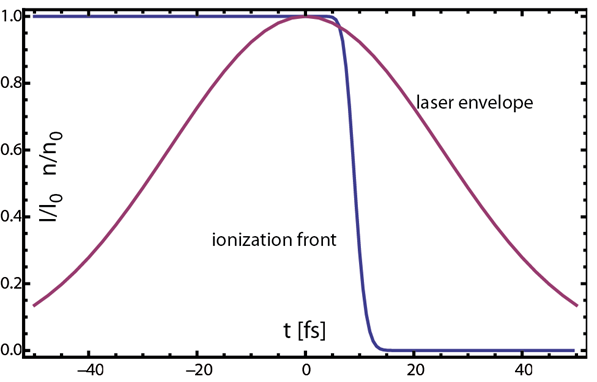
\includegraphics[width=0.2\textwidth]{theory/images/raw/Ionization_front.png}
\end{figure}


\begin{figure}
\begin{center}
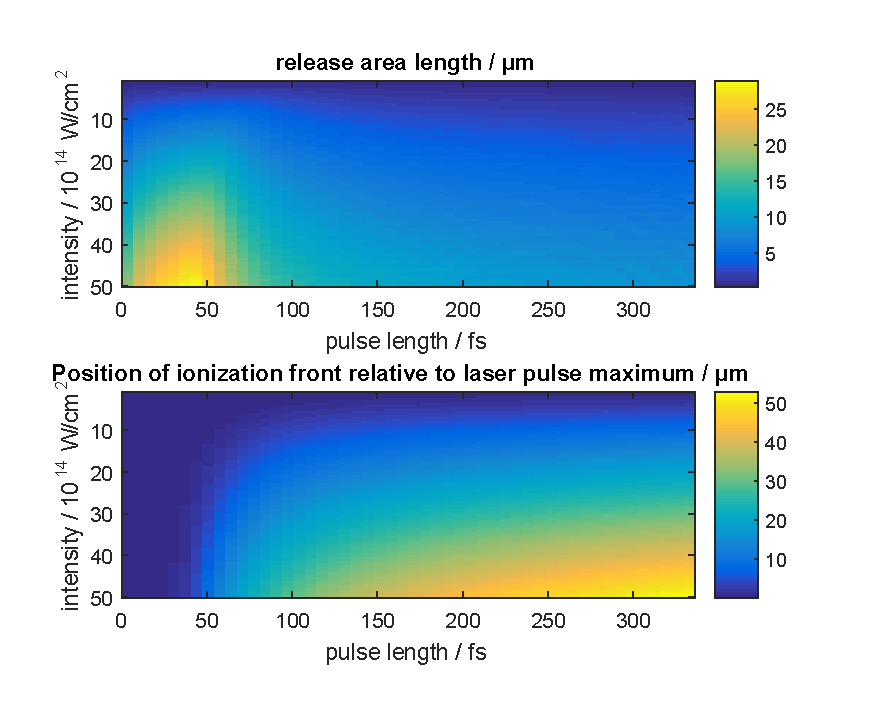
\includegraphics[width=0.5\textwidth]{theory/images/edited/IonFrontVariation.pdf}
\end{center}
\end{figure}



\subsubsection{emittance preservation}
why don't you ... look at space charge effect to estimate required gamma/acceleration and focusing forces for emittance preservation ? Try looking at Pak's thesis and this emittance paper that claims one needs a fast acceleration, but knows nothing about Trojan Horse yet.
\section{Acceleration methods in PWFA}
The strong accelrating fields in PWFA can be harvested with a variety of methods. They differ in experimental complexity, demand towards drive beam 



\subsection{External injection - Double bunch}
External injection is the least complex PWFA setup and is also the method that has been demonstrated much earlier than other methods. The basic idea is that a plasma wake is set up by an electron beam, electrons - either from the same electron beam or by a trailing electron beam - are accelerated, if they are at the right phase with respect to the wake.

The first experimental realization of a PWFA was established in 1988 at the Argonne advanced accelerator test facility (AATF)\cite{rosenzweig1988experimental}. With a method successfully applied to measure the wake fields in accelerating structures
a $2-3\ \mathrm{nC}$ electron beam with a rms bunch length of $2.4 \mathrm{mm}$ was used to drive a wake in a $33\ \mathrm{cm} $ long plasma at a density of the order of $ 10^{13}\ \mathrm{cm}^{-3}$. The driving bunch was trailed by a low-charge witness beam with variable delay to scan the wake fields.
The oscillating nature of the wake fields was well measured with a maximum accelerating gradient of $1.6\ \mathrm{MeV/m}$. 
With a higher driver witness beam charge of $4\ \mathrm{nC}$ \cite{figueroa1988direct} it was possible to show a non-linear wake with an accelerating gradient of $5.3\ \mathrm{MeV/m}$. 

In 2006 at the Final Focus Test Beam Facility (FFTB) at the Stanford Linear Accelerator Center (SLAC) the blow-out regime was finally reached as described in \cite{blumenfeld2007energyDoubling}.
A $42\ \mathrm{GeV}$ electron beam with a spot size of $10\ \mathrm{\mu m}$ and rms bunch length of $~15\ \mu\mathrm{m}$ propagated through a $85\ \mathrm{cm}$ Li oven. The shorter, high current bunch now allowed for driving a wake in a much higher plasma density of $2.7\times 10^{17}\ \mathrm{cm}^{-3} $ in the blowout regime. Thanks to the extremely high wake field gradient of $52\ \mathrm{GeV/m}$ which effectively accelerated part of the electron beam to up to $85\ \mathrm{GeV}$.

The successor experiment to the plasma experiments at the FFTB is the Facility for Advanced Accelerator Experimental Tests (FACET)\cite{clarke2012facet}. Several double-bunch experiments have been successfully conducted.  
At FACET the double-bunches are produced by accelerating one long electron bunch all the way to the final chicane. 
While the chirped bunch is dispersed, the central part is cut out by a mask which results in a scrape in the current profile  \cite{hogan2010FACET}. This method has the advantage that the transport of the beam along the LINAC is only required for one bunch.
Efficiency and beamloading effects were studied in \cite{litos2014high} and recently at FACET a double-bunch acceleration of positrons in a positron-driven wake was demonstrated by shaping the transverse plasma shape to a hollow channel, which effectively avoids any transverse fields that would otherwise defocus the positrons \cite{ThesisGessner}.
\subsection{Density Downramp injection}

\subsection{Plasma Torch}
\cite{PlaTo,PlaTo2}
%\subsection{Transverse injection ?}
\subsection{ionization injection}
In all previously outlined injection types, electrons to be accelerated in the wake are at a nonzero velocity when injected, which is an advantage as regards the requirements on the wakefield gradient. Ionization injected electrons are in a bound state until they are released to continuum inside the wake. This from a physics standpoint requires the plasma to only be partially ionized when the wake is excited and from an engineering stand point ionization levels that are sufficiently distinct in their ionization rates to ensure a controlled ionization. We will further use the term Low ionization threshold (LIT) medium for the part to be ionized in order to drive the wave in it and High ionization threshold (HIT) medium for the part that originates the injected witness beam electrons. Of course, HIT and LIT medium can be the same, by making use of different ionization levels. If, however, HIT and LIT are different gases as e.g. H$_2$ and He, their gas density ratio becomes a handy degree of freedom to control the injected charge.
Experimentally in \cite{Navid_distributed_PRL} ionization ionjection was shown in a Rb oven. The electron beam head electric fields were used to ionize $Rb\rightarrow Rb^+$, while the drive beam tails' field overlapped with the wake electric fields were strong enough to ionize $Rb^+ \rightarrow Rb^{2+}$ and inject the. This method of injection electrons is conceptually comparable to ionization injection, where the driving laser pulse fields are strong enough to ionize several ionization levels with injection at the back of the laser or in other words the front of the wake\cite{Pak_Ion_InjectionPRL2010}.

In \cite{Ossa_Rake_PRL2013} and \cite{MartinezdelaOssa2014231} with theory and simulations a setup was examined where only the back of the wake had sufficiently high fields to ionize the HIT medium and combined with the concept of the trapping potential as described in section (\ref{sec:Theory_Trapping}). It could be shown that the combined requirements for trapping, i.e. the overlap of the ionization region and the trapping region, confine the possible electron source which enables the generation of low emittance electron beams ($\epsilon_x=1.5\ \mathrm{\mu m}$) 




%\begin{figure}

%\end{figure}
\subsection{Trojan Horse injection}
\label{sec:Theory_TrojanHorse}
The underdense photocathode or Trojan Horse injection is one of the most complex injection techniques. It was proposed by B. Hidding in \cite{Hidding_PRL_2012}. Neither the wake nor the beam electric fields are sufficient to ionize the HIT medium. Instead this is the duty of an additional short-pulse laser pulse, trailing the driving electron beam. Given full control over laser-to-electron beam alignment and synchronization, it is possible to ionize and release electrons wherever in the wake it deems necessary. It could be shown that a release in the potential minimum, i.e. the zero-crossing of the wake is particularly advantageous, because the electron acceleration to relativistic speed is extremely rapid ($\approx \frac{\lP}{2c}$) and the bunch compression is maximum at this injection position. Furthermore the emittance of Trojan Horse injected electron beams can be very low on the order of a few $\epsilon_\mathrm{rms}\approx 10^{-8}\ \mathrm{m rad}$. The reasons for that lie to one part in the ionization method. A typical $800\ \mathrm{nm}$ Ti:Sa few fs laserpulse only needs a peak intensity of $10^{15}\ \mathrm{W/cm^2}$ to ionize a HIT medium as e.g. $He \rightarrow He^+$. The normalized vector potential $a_0 = \frac{\qE E_0}{\mE c^2} = 0.022<<1$ implies that no ponderomotive force can be expected that would impose an inital transverse momentum to the released electron bunch wo that the transverse momentum is basically determined by the HIT gas temperature. 
A detailed theoretically supported PIC simulation parameter scan in \cite{xi2013hybrid} examined scalings between witness emittance and brightness and laser beam parameters as beam waist $w_0$, pulse length and peak intensity. A indifference towards pulse length as well as an emittance increase with $w_0$ and intensity could be demonstrated.

In \cite{hidding2014ultrahigh} a detailed comparison between laser and electron beam driven wakefield acceleration was drawn.
 
\section{Trapping behaviour for the Trojan Horse Injection}

With $E_{bind}$ being the binding energy and $U_p=\frac{q^2 I}{2 m_e \epsilon_0 c \omega^2}$ being the ponderomotive energy 
\begin{equation}
\gamma=\sqrt{\frac{E_{bind}}{2U_p}}
\end{equation}


\section{Influence of the ionization behaviour}



	Here it is to be described how for TH the co-moving frame is advantagous. dependence of ionization front to 
	create witness beams.
	Image of Ionization front.
	
	
	%\subsection{Rake injection}


	
\subsection{Downramp assisted Trojan Horse}

\section{numerical modeling of Trojan Horse injection}

\subsection{Movement of ionization front}
\subsection{emittance growth from space charge}
\subsection{Laser parameter variations}
	

\chapter{Simulations}
\section{Start-to-End simulations for a Trojan Horse at FlashForward experiment}
\section{The trapping potential}
\section{plasma density profile optimisation}
\subsection{Density Downramp facilitated Trojan Horse Acceleration}

In %\cite{Fub_PRL_downramp}
 wird beschrieben, wie sich ein negativer Dichtegradient auf die in einer Plasmawelle getrappten Elektronen auswirkt.
Ausgangspunkt ist dabei die LWFA mit der Annahme, dass bei konstater Elektronendichte der Laserpuls, sowie die Bubble sich mit c bewegen.\\
Die Welle bewege sich in z-Richtung.\\
Die L\"ange der bubble ist Abh\"angig von der Plasmadichte $n$. Da sich diese \"uber eine downramp von $n_i$ auf $n_f$ verringert, vergr\"o\ss ert sich auch die bubble \"uber diese Strecke.
Sei $$\xi=z-ct$$ die Position relativ zum Laserpuls. $\xi<0$ beschreibt die Position eines Elektrons in der Bubble hinter dem Laserpuls.
Das Elektron bleibt am gleichen Ort relativ zur Bubblestruktur, aber die Bubble ver\"andert sich. Die Phase der Bubble ver\"andert sich von 
$$\Psi_i=\frac{\omega_{pi}}{c}\xi$$ nach
$$\Psi_f=\frac{\omega_{pf}}{c}\xi$$
mit der Phasendifferenz:
$$\Delta\Psi=\Psi_f-\Psi_i=\Psi_i[1-(\frac{n_f}{n_i})^{1/2}]$$
Die entsprechende Phasengeschwindigkeit errechnet sich aus 
$$v_p=-\frac{\frac{\partial \Psi}{\partial(ct)}}{\frac{\partial \Psi}{\partial z}}=\frac{c}{1+\frac{1}{2\omega_p(z)n(z)}\frac{\partial n(z)}{\partial z}\xi }$$

$$\Delta \lambda_\mathrm{p} \propto (e^{\frac{1}{2}C_\mathrm{ramp}z_1}-e^{\frac{1}{2}C_\mathrm{ramp}z_2}) $$
$$\approx \frac{1}{2}C_\mathrm{ramp}(z_1-z_2)  $$
\subsection{density transition injection suppression}
See paper by Suk

\section{Laser Beam shaping for optimisation}
\subsection{my beamloading description}
\subsection{beamloading in theory}

\subsection{beamshaping in reality}
-pulse-shaping by spatial light modulator(SLM) (Meshulach adaptive real-time fs pulse shaping)

\section{Magnetic Field facilitated Trojan Horse Acceleration}





%\chapter{The FACET E210 Experiment}
In 2014 the experimental campaign  for demonstrating the proof-of-concept of Trojan Horse injection (see \ref{sec:Theory_TrojanHorse}) started at the Facility for Advanced Accelerator Experimental Tests (FACET) at the SLAC national laboratory as the experiment E210. It was a collaborative effort with researchers from the University of Hamburg, University of California Los Angeles (UCLA), University of Strathclyde Glasgow and Radiabeam technology with a devoted support from the SLAC personnel. The FACET experiments had to be designed to be non-excluding, which led to a fruitful joint learning process between several groups.
It is fair to say that E210 was one of the most complex and accuracy-wise most demanding experiments conducted so far at FACET. 
Several steps were required in improving the overall setup, until the experiment was eventually successful.
The most crucial obstacles to overcome were timing and alignment between two laser arms and the electron beam.
The timing requirements between the electron beam and the pre-ionization laser are rather soft as long as the pre-ionization occurs before the arrival of the electron beam an with a timing difference less then the recombination time (ns-µs range). However, proper control over relative time-of-arrival between the injection laser and the electron beam required - in principal - control over timing on the order of $10\ \mathrm{fs}$. With an expected timing jitter in the range of $200\ \mathrm{fs}$ the best solution here was to accurately measure the relative TOA with an electro-optical sampling (described in\ref{sec:EOS}) to determine the injection properties from the data, rather than hope for live-control. 
For finding the synchronization ($t_0$) as well as fine-alignment between electron beam and injection laser, a newly observed effect on the plasma glow described in \ref{sec:Plasma_Glow} was measured and applied.

\section{The FACET experimental setup}
\subsection{LINAC}
\subsection{The FACET laser system}
Good description of FACET laser system in \cite{Green_FACET_Laser_PIOP}
\subsection{Imaging spectrometer}

\subsection{Laser energy calibration}
The FACET laser system ...
The energy that can be used on target of the OAP is controlled at two points in the laser-beamline.
At each point a cube-polarizer is surrounded by two  $\lambda/2$-waveplates, where the upstream one is motorized.
The main energy waveplate is located in the laser-room and the probe-energy waveplate is located in the tunnel area shortly after the split between main laser path and probe laser path at the main sampler, which means that the probe laser energy is determined by both waveplate settings while the main laser energy is set by the main laser energy waveplate only. From the power-meter in the laser-room, that measures shot-by-shot laser pulse energy, all the way down to the tunnel a variety of optical components are used until the laser is finally focused onto the 
The typical shot-to-shot laser energy jitter  is $\approx 5 \%$ FWHM.

Manta Cameras: \cite{GigE125_datasheet}

\begin{figure}[htbp]
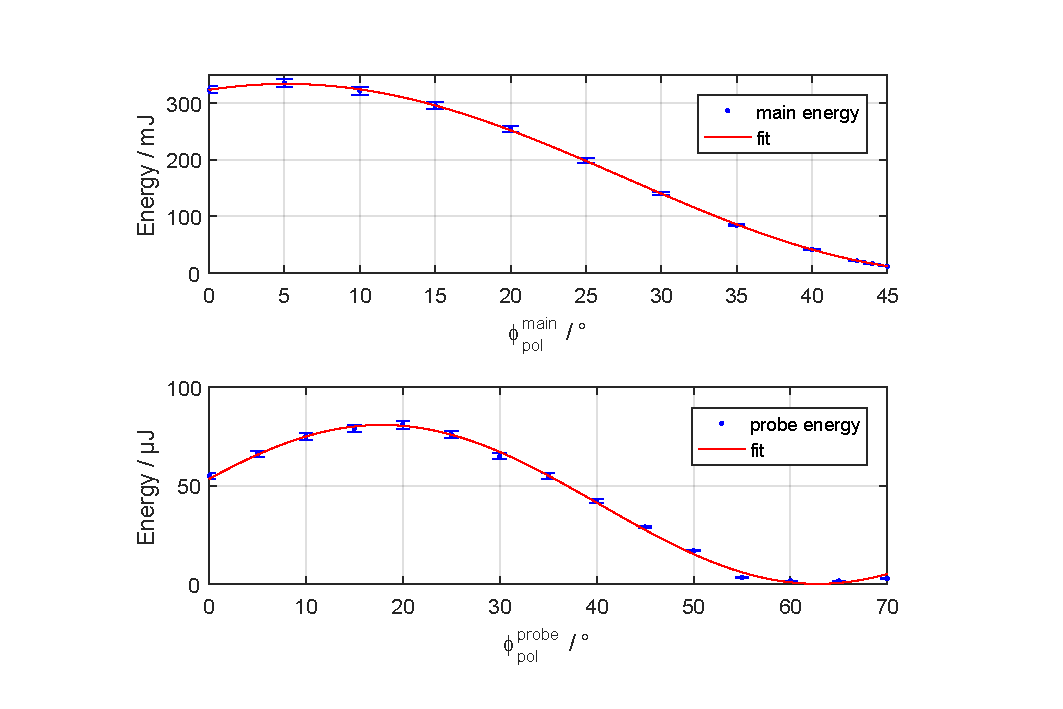
\includegraphics[width=0.9\textwidth]{experiment/images/edited/waveplate_calibration.pdf}
\caption{Laser energy calibration for main energy waveplate (upper plot) and probe energy waveplate (lower plot)}
\label{img:LaserEnergyCalib}
\end{figure}

All measured losses in optical components combined with the fitted functions for the waveplate energies (see figure \ref{img:LaserEnergyCalib}) combined give the on target energy applicable by axilens and OAP respecively.
\begin{align*}
 W_\mathrm{Laser}^\mathrm{OAP} &= W_\mathrm{Laser}^\mathrm{Laserroom}\times 1.25\times10^{-2}\\ 
 &\times\big( 0.994 \cos^2((\phi_{pol}^{main}-5.11\degree)) +1.16\times 10^{-3}\big)\\
  &\times \big(0.998 \cos^2((\phi_\mathrm{pol}^\mathrm{probe}-17.8\degree )) +1.62\times 10^{-3}\big)
\end{align*}

\begin{align}
 W_\mathrm{Laser}^\mathrm{Axilens} &= W_\mathrm{Laser}^\mathrm{Laserroom}\times 0.253\\
  &\times\big( 0.994 \cos^2((\phi_\mathrm{pol}^\mathrm{main}+66.9\degree)) +1.16\times 10^{-3}\big)\\
\end{align}
This means that for a typical laser energy output of $500\, \mathrm{mJ}$ a maximum energy of $6.2\, \mathrm{mJ}$ on OAP target and $125.9\,\mathrm{mJ}$ on axilens could be used.


\section{Electro Optical Sampling (EOS)}
\label{sec:EOS}
Electro-optical sampling is a method that allows for determining time-differences in Time-of-arrival between a laser-pulse and a Thz-source, as e.g. an ultra relativistic electron-beam, by exploiting the properties of optically anisotropic crystals and has been shown to be able to measure sub-picosecond electron bunches \cite{YanX_EOS_PRL2000}.

Electromagnetic waves, propagating through anisotropic crystals perceive a difference in dielectric permitivity $\epsilon_\mathrm{r}$, depending on entrance angle and polarization of the wave, which is why in a more general way the dielectric properties need to be addresses with the dielectric permitivity tensor  $\hat{\epsilon}$.
This is equivalent to a polarization-depending index of refraction, a property known as birefringence, which leads to a polarization-dependent phase velocity of light inside the crystal. 
A laser at the correct incident angle with respect to an anisotropic crystal will therefore notice a phase shift between different planes of polarization which leads to an overall change in the laser polarization, depending on the phase shift strength and the crystal size. 
Electro-optical crystals change the orientation of the dielectric permitivity tensor when an external electric field $\vec{E}_\mathrm{ext.}$ is applied.
The strength of this effect can be illustrated by taylor-expanding the impermeability tensor 
\begin{equation}
\hat{\eta}=\hat{\epsilon}^{-1}
\end{equation}
for small external electric fields $\vec{E}_\mathrm{ext.}$ to
\begin{equation}
\eta_{ij}=\eta_{ij}(0)+r_{ijk}E_k+s_{ijkl}E_k E_l+...\ .
\end{equation}
The linear dependency on the electric field strength is called Kerr-effect with $r_{ijk}$ being the Kerr-coefficient. 
The Pockels effect with the Pockels coefficient $s_{ijkl}$ describes quadratic dependency.
In the context of this work and the described experiment only two elctro-optical crystals were used, GaP and ZnTe. 
As both of them are packed in a zincblende geometry, which does not obtain an inversion center, the electro-optic effect is dominated by the Kerr-effect.

\subsection*{EOS setup}
In order to measure the relative time-of-arrival between electron bunch and laser pulse an Electro optical sampling (EOS) was set up as a non-destructive shot-by-shot diagnostic.

In this experiment the crystal is located in close proximity (few mm distance) to the electron beam axis. Due to the high $\gamma_\mathrm{b} \approx 42000$ , the beam electric field is strongly lorenz-contracted and can be assumed to temporally only extend for the length of the electron beam. Consequently the electric field applied to the crystal and with that the induced birefringence are only active while the electron beam passes by the crystal.  
Figure \ref{img:EOS_Setup} depicts the setup.
A linear polarized laser pulse (red), a pickup of the probe beam, traverses the crystal with an angle of $~ 45\degree$ with respect to the electron beam axis (green). The laser beam is collimated with a transverse diameter of $~ 1 cm $ and completely illuminates the crystal. For a better signal-to-noise ratio, an additional polarizing filter was installed prior to the picnic basket chamber. After the chamber follows a cross-polarized filter, which can remotely be rotated for alignment purposes.

During the measurement only the polarization of that transverse part of the laser which propagates through the crystal at the very moment in which the electron beam' electric field induces the birefringence will be rotated and not be filtered by the polarizing filter further  downstream the laser beam path. As a result the signal has the form of a line as seen in figure \ref{img:EOS_Signal} with a horizontal position linearly corresponding to the relative TOA.

\begin{figure}[htbp]
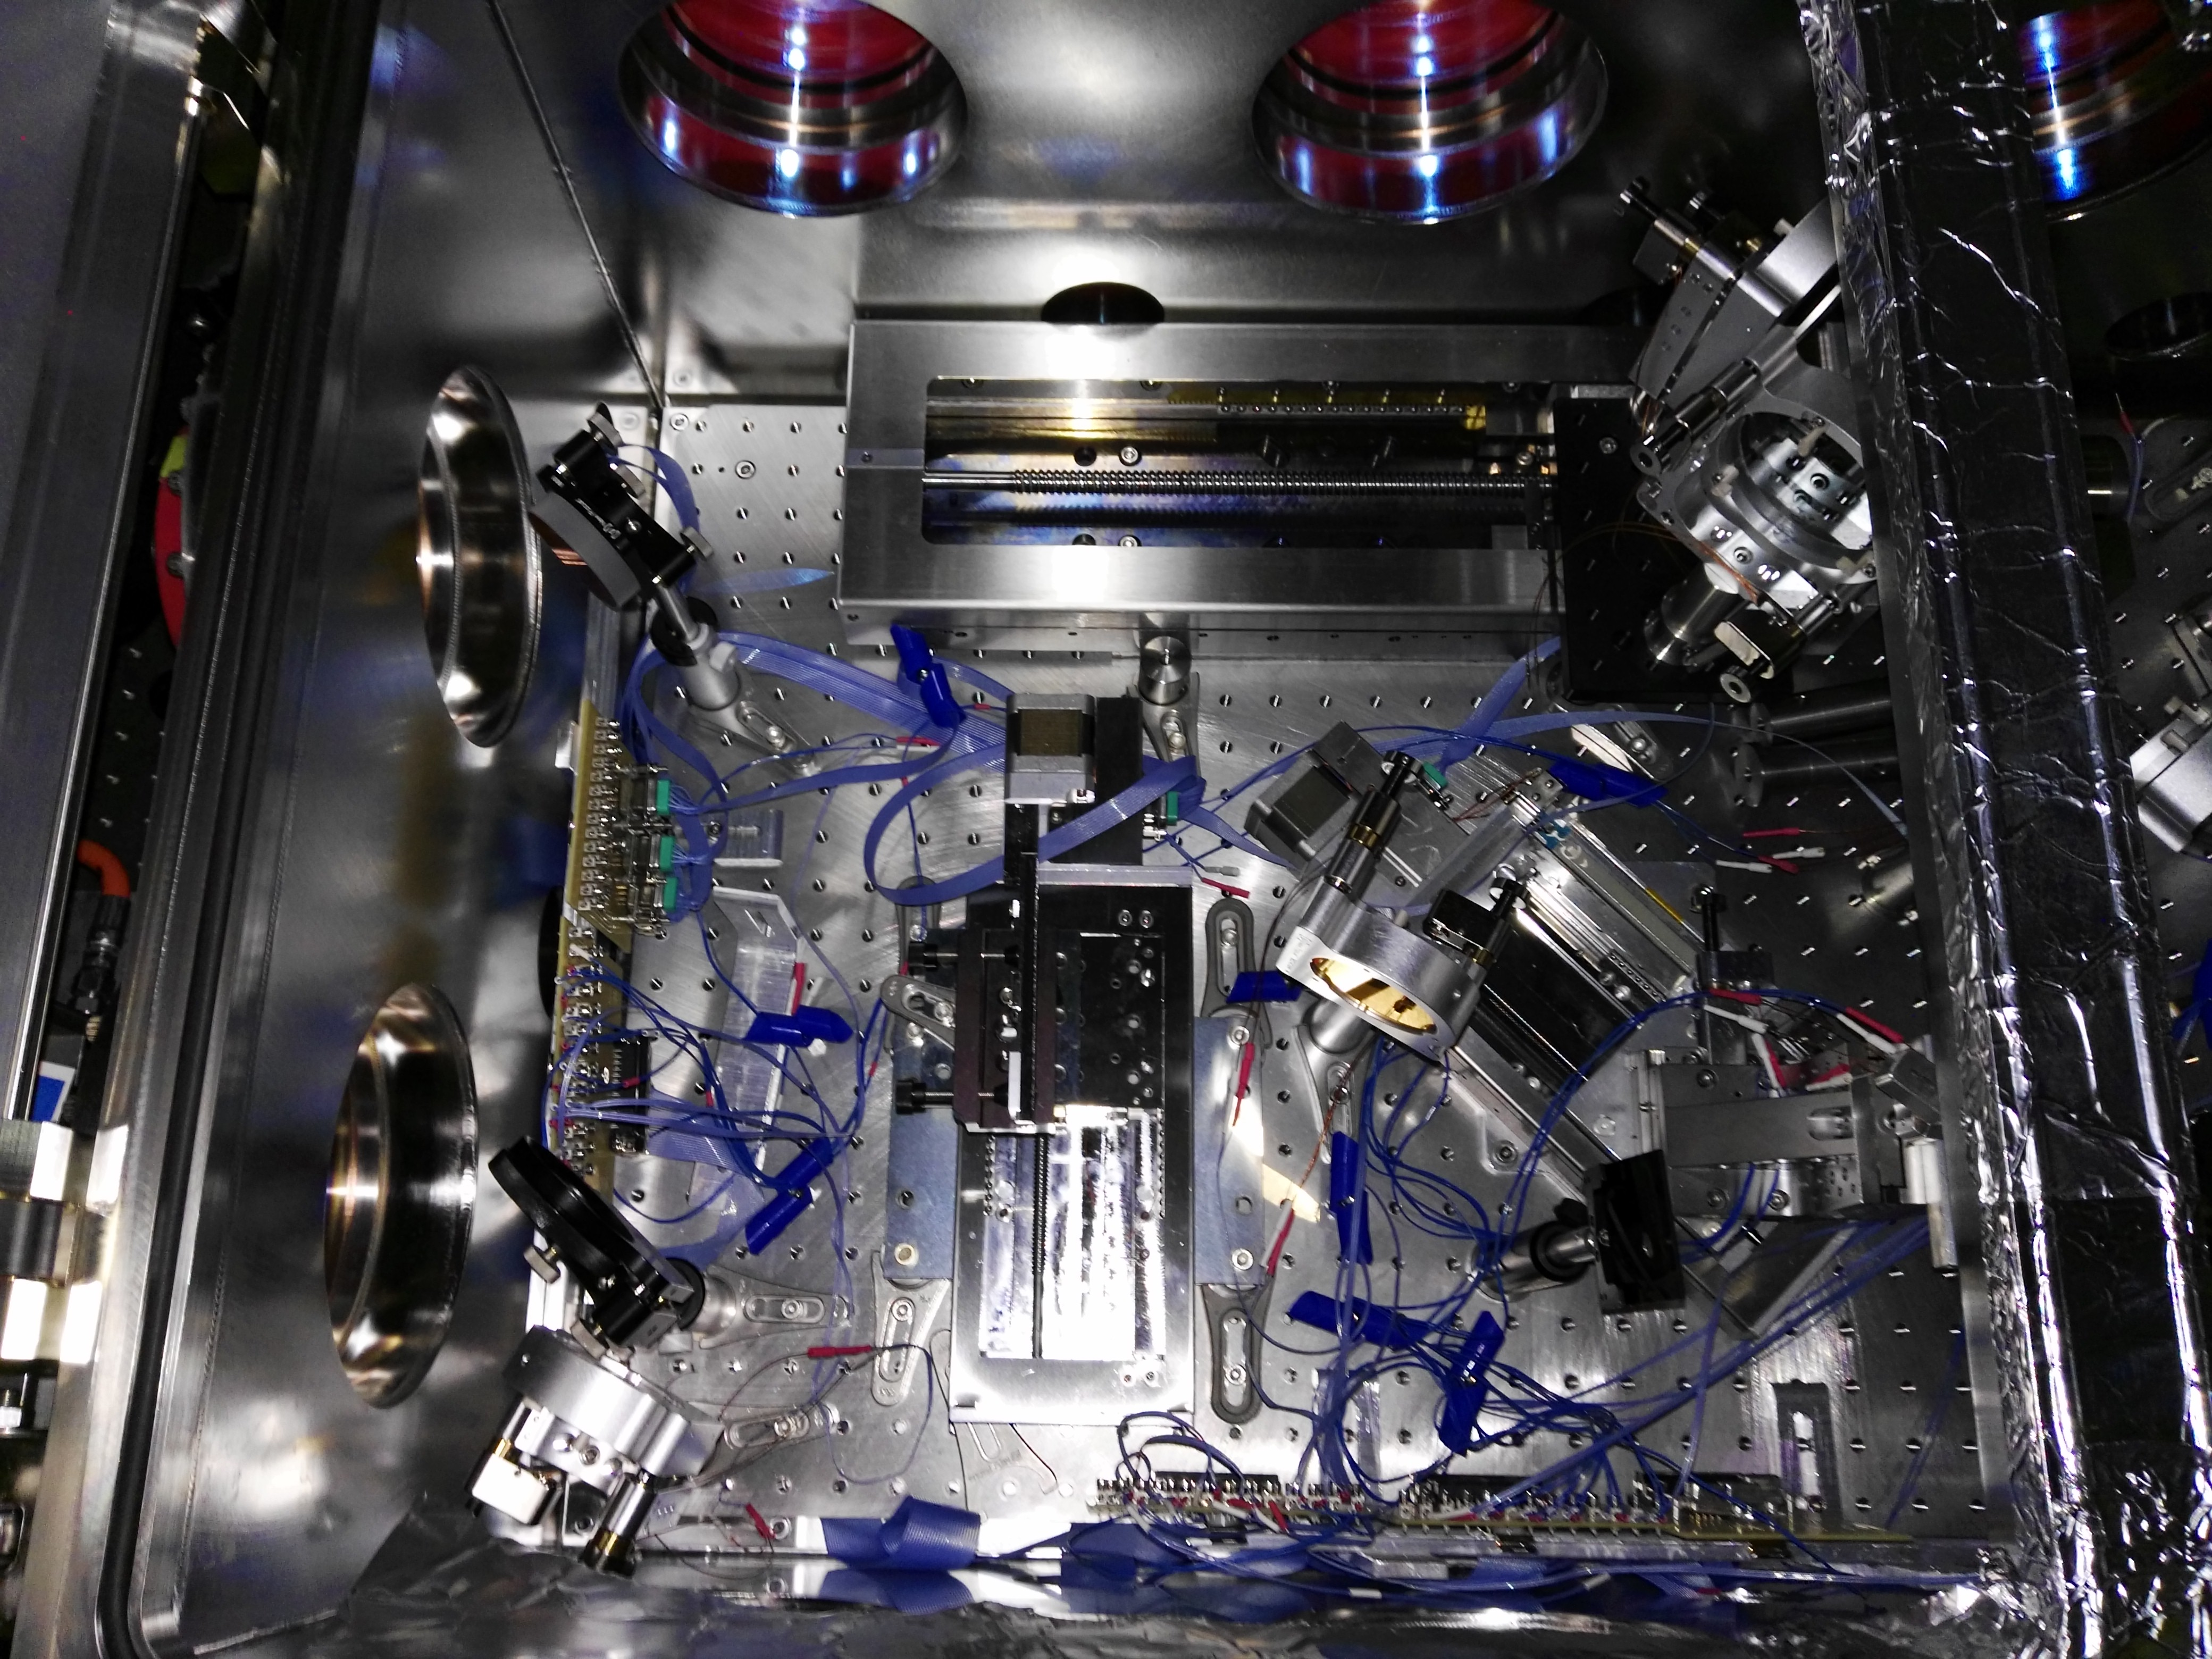
\includegraphics[width=0.5\textwidth]{experiment/images/edited/EOS_setup.pdf}
\caption{Setup of upstream electro-optical sampling inside the picnic basket chamber. Electron beam (green) and EOS laser (red) co-propagate in a small angle }
\label{img:EOS_Setup}
\end{figure}

The crystal plate is oriented perpendicular to the electron beam axis to minimize temporal overlap and the laser has an $\approx 40°$ angle with the electron beam which enables a correlation between signal position i.e. the part of the laser with rotated polarization and relative timing.

The entire ladder supports a YAG crystal to find the electron beam axis, a $500\ \mathrm{µm}$ thick ZnTe for broad timing scans and GaP with $100\ \mathrm{µm}$ thickness for fine resolution.
A detailed description of the physics involved in the application of electro-optical crystals as TOA and bunch length diagnostic can be found in \cite{BerndSteffenPhD}.


\begin{figure}
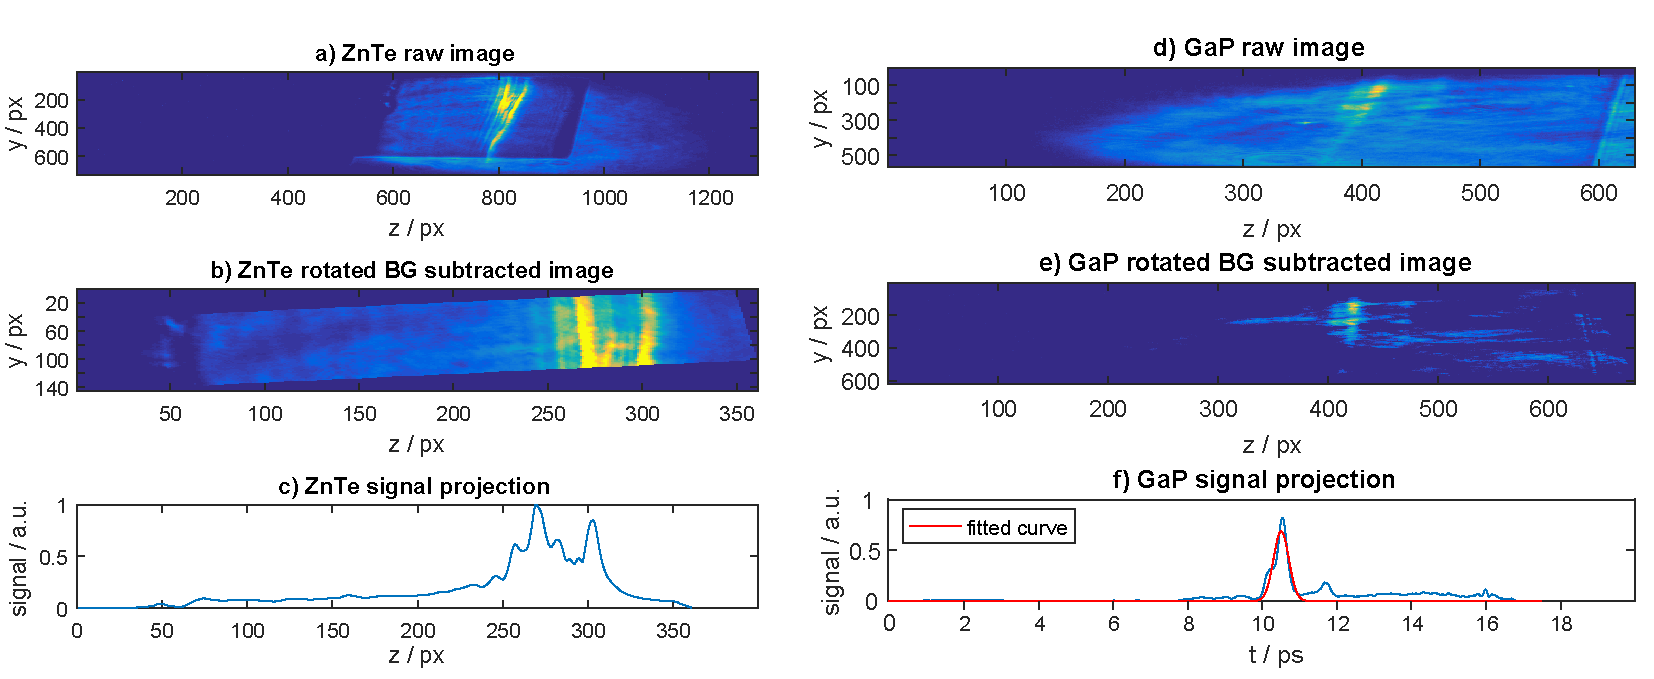
\includegraphics[width=1.0\textwidth]{experiment/images/edited/EOS_Signal.pdf}
\caption{EOS signal}
\label{img:EOS_Signal}
\end{figure}
\subsection*{EOS calibration}

\begin{figure}
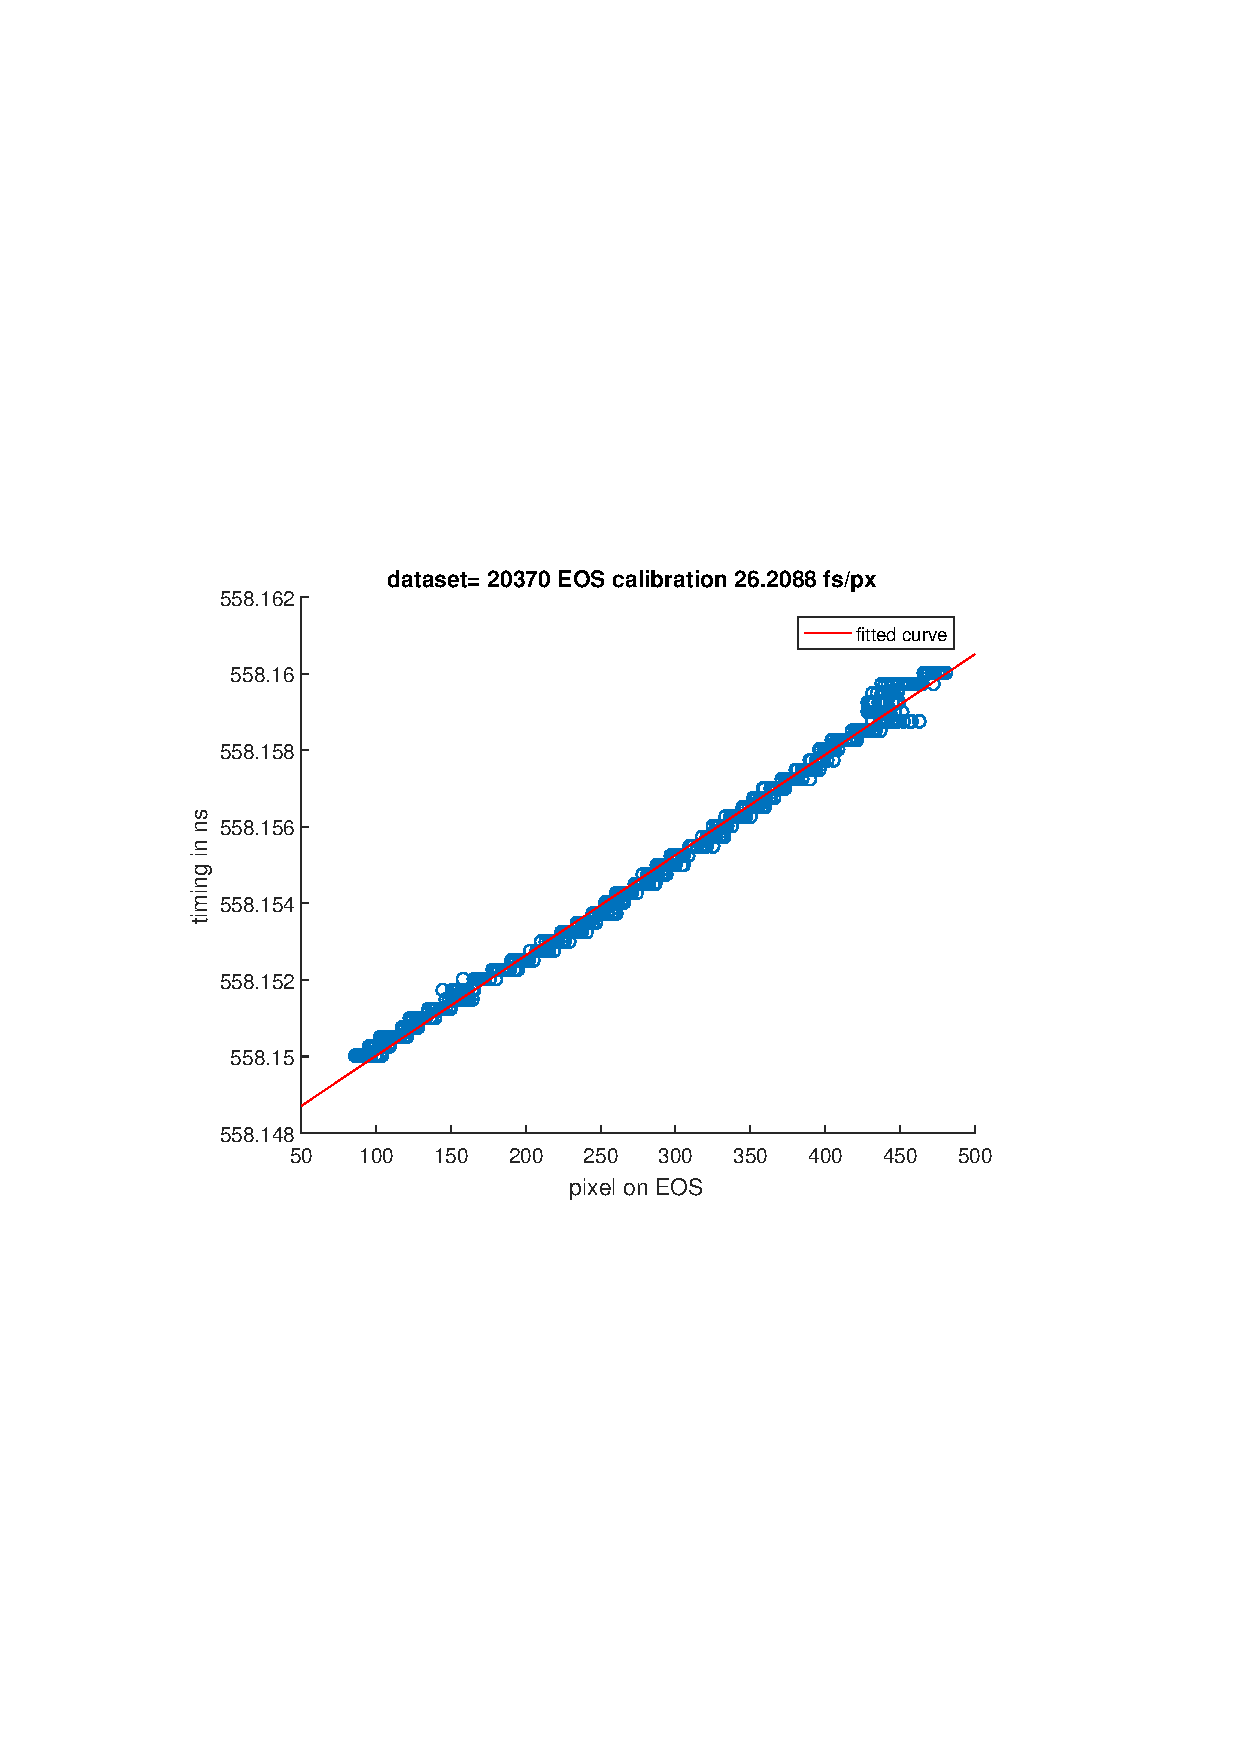
\includegraphics[width=1.0\textwidth]{experiment/images/raw/20370_EOS_calibration.pdf}
\caption{Typical EOS calibration}
\label{img:EOS_Calib}
\end{figure}
For the calibration of the EOS timing, scans were performed in which the arrival time of the laser was altered by changing its
path length. 

%\section{Torch kick}
%\begin{figure}[htbp]
%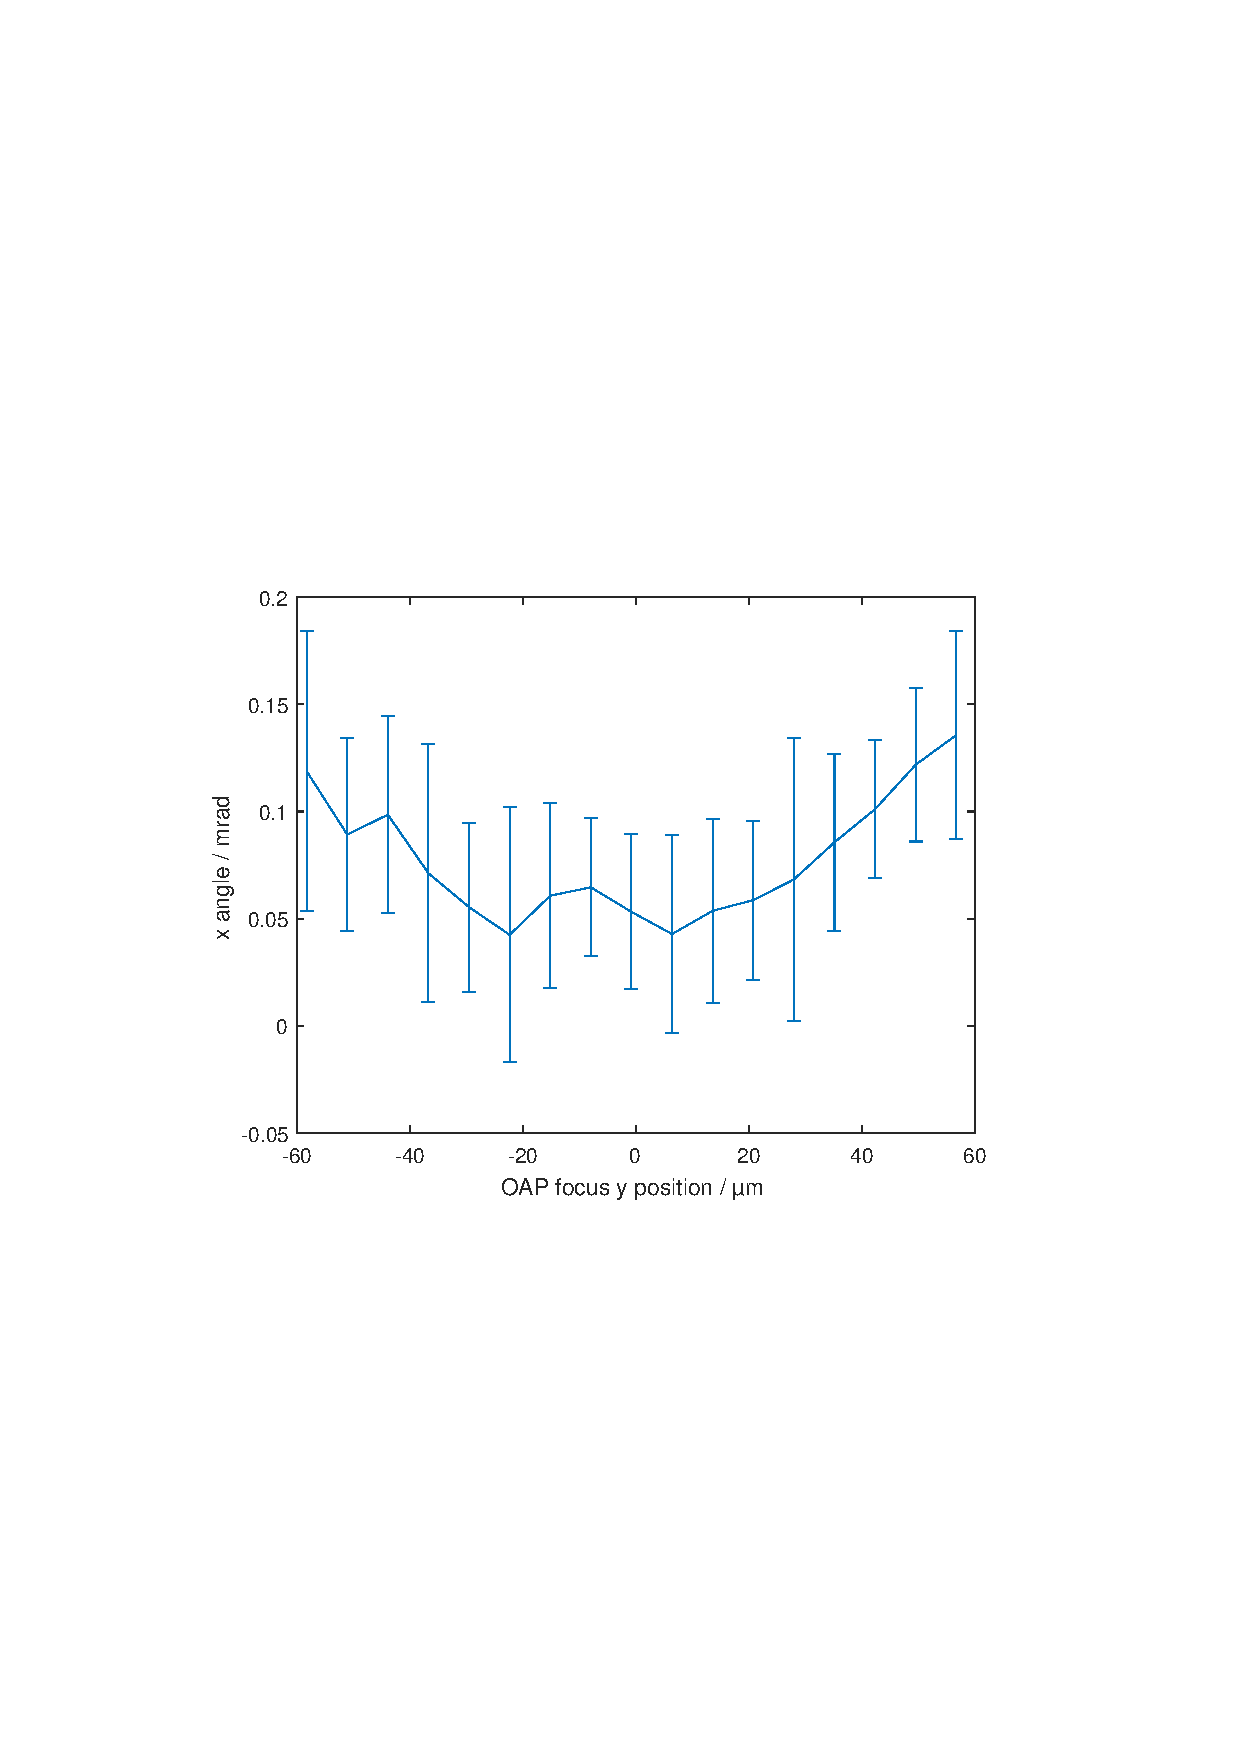
\includegraphics[width=0.9\textwidth]{experiment/images/raw/Torch_rollscan.pdf}
%\caption{'test'}
%\label{img:TochKick}
%\end{figure}
\newpage
\section{Ionization test}

\section{Plasma glow diagnostic}
\label{sec:Plasma_Glow}
One huge advantage of the hydrogen FACET setup compared to the oven setup is that now several view ports allow for observing the interaction or \ref{Facet_setup}.

The plasma glow diagnostic as a very simple tool, that turned out to be extremely helpful in controlling the 
alignment and synchronization of the experimental setup. The main idea is to have a camera integrate over the recombination light. It was observed that this 

\begin{figure}[htbp]
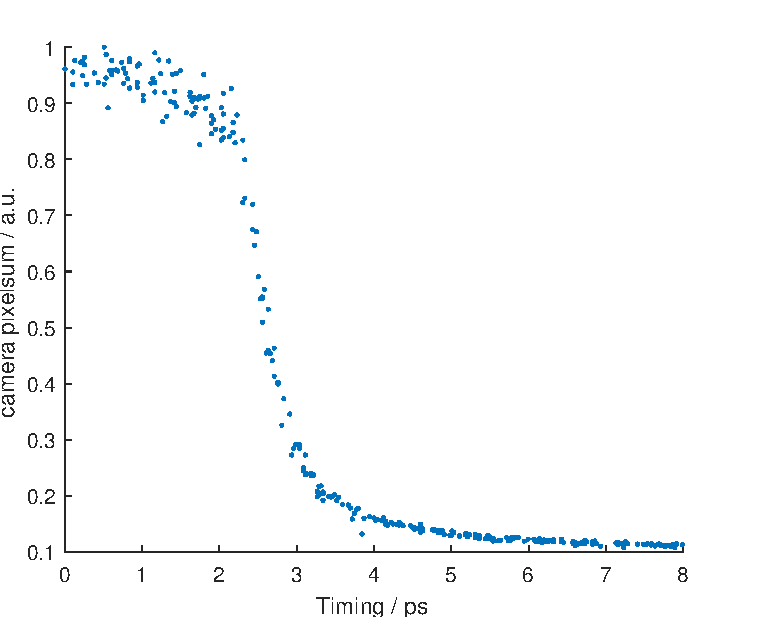
\includegraphics[width=1\textwidth]{experiment/images/raw/PlasmaGlow_20384_scatter.pdf}
\caption{Relative electron beam to injection laser timing scan. The pixel counts measured by the cube 3 vertical camera with a 656$\pm$10 nm  band-pass filter are sorted by the EOS. evaluation.}
\label{img:PlasmaGlowTimingOAP_H2He}
\end{figure}

Figure \ref{img:PlasmaGlowTimingOAP_H2He} shows the plasma glow accumulated intensity at the wavelength 656$\pm$10 nm , sorted by relative time-of-arrival between electron beam as measured by the EOS. The transition between a situation where the injection laser arrives earlier than the electron beam and vice versa is around $1\ \mathrm{ps}$ wide, which sufficiently fulfills the requirements to find a range of synchronization as the total range of the EOS crystal is around 20 ps ???.
During the data acquisition the electron beam charge was $3.1\pm \ 0.17\ \mathrm{nC}$. 

\begin{figure}[htbp]
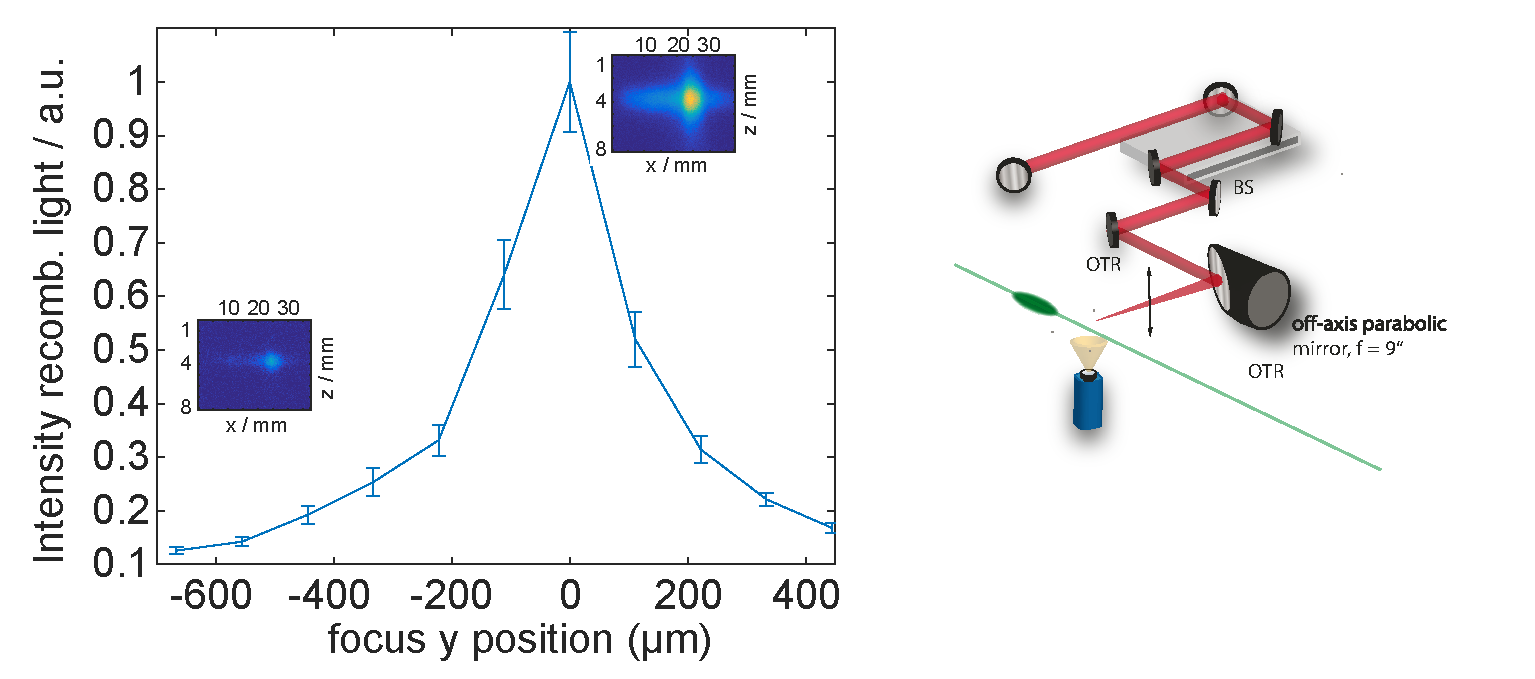
\includegraphics[width=0.5\textwidth]{experiment/images/edited/Plasma_Glow_roll.pdf}
\caption{Plasma glow in 7.8 torr $\mathrm{H}_2$ ( $n_\mathrm{e}=5\times10^{17}\mathrm{cm}^{-3} $) measured by vertical camera in cube 3. The injection laser off-axis parabola roll is scanned. The vertical plasma position is evaluated by the focus diagnostic.}
\label{img:PlasmaGlowRoll}
\end{figure}



\subsection*{Result:}
With the 
\section{Result: Plasma Torch injection}
\section{Result: Trojan Horse injection}
\bibliography{lib}
\bibliographystyle{plain}    
\end{document}